%This is a LaTeX template for homework assignments
\documentclass{article}
\usepackage[utf8]{inputenc}
\usepackage{algorithmic, algorithm, amsmath, color, graphicx, hyperref}
%\usepackage{algpseudocode}
%\usepackage[named]{algo}

\begin{document}

\title{CSCE 626 Programming Assignment 2}
\author{Jordan Cazamias}
\date{3/30/2015}
\maketitle

\section*{References Consulted}

\begin{itemize}
\item NVIDIA Parallel Prefix Sum with CUDA: \url{http://http.developer.nvidia.com/GPUGems3/gpugems3_ch39.html} 
\item CSCE 626, Experimental Evaluation: \url{https://parasol.tamu.edu/~amato/Courses/626/lectures/CSCE626-Amato-LN-ExperimentalSetup.pdf}
\end{itemize}

\textit{By submitting this assignment I certify that I have documented in the assignment itself all the sources that I consulted regarding this assignment, and that I have not received or given any assistance that is contrary to the letter or the spirit of the collaboration guidelines for this assignment.}

\section{Introduction}
The prefix sum algorithm is an essential tool in the parallel programmer's toolbox.  It is often the core algorithm that drives other, more sophisticated algorithms that range in many different applications.  As such, having an efficient implementation of the prefix sum algorithm will have a wide impact on the overall performance of algorithms.  In this analysis, three implementations of the prefix sum algorithm are presented, implemented, and tested under various conditions.  The first is simply the naive sequential prefix sum algorithm, used as a base for comparison.  The second is a shared-memory parallel implementation using OpenMP.  The third is a message-passing implementation using MPI.  In determining which algorithm performs the best under what conditions, many factors will be considered such as scaling, speedup, and how the experimental results stack up to the theoretical results.

\section{Theoretical Analysis}

\subsection*{OpenMP Algorithm}
The OpenMP implementation was adapted from the first programming assignment, and originally came from an NVIDIA article about designing a work-optimal prefix sum algorithm.  The pseudocode is shown below:
\begin{algorithm}[H]
\caption{PrefixSum\_OpenMP($X$)}
\begin{algorithmic}[1]
\STATE $id \gets $ get process id // Presumed $id \in [1,p]$
\STATE $n \gets $ size of $X$
\item[]
\STATE // Up Sweep
\FOR{$i = 1$ to $\log(n)$}
	\STATE $step \gets 2^id$
	\STATE // Run loop in parallel
	\FOR{$j = step-1$ to $n$ step $step$}
		\STATE $X[j] \gets X[j] + X[j - step/2]$
	\ENDFOR
\ENDFOR
\item[]
\STATE // Down Sweep
\FOR{$i = \log(n)-1$ to $1$}
	\STATE $step \gets 2^id$
	\STATE // Run loop in parallel
	\FOR{$j = step-1$ to $(n - step/2)$ step $step$}
		\STATE $X[j + step/2] \gets X[j + step/2] + X[j]$
	\ENDFOR
\ENDFOR
\end{algorithmic}
\end{algorithm}

For each sweep, the cores collectively evaluate $n/2 + n/4 + \cdots + 1 = O(n)$ array slots, and thus performs $O(n) work$.  This amounts to $O(n/p)$ complexity for the time.  Due to the experimental setup, we will assume that $p = O(1)$ rather than $O(n)$.  As such, the OpenMP algorithm will run in $O(n)$ time and perform $O(n)$ work.


\subsection*{MPI Algorithm}
The MPI Algorithm is also adapted from the first assignment.  Unlike the OpenMP algorithm, however, the MPI algorithm is implemented from a core-centric view rather than a global view.  So, the pseudocode below describes what is performed at the individual core level rather than at the global level:

\begin{algorithm}[H]
\caption{PrefixSum\_MPI($X$)}
\begin{algorithmic}[1]
\STATE $id \gets $ get process id // Presumed $id \in [1,n]$
\STATE $p \gets $ number of processors
\STATE $n \gets $ problem size
\STATE $m \gets $ size of problem chunk assigned to node // Roughly $n/p$
\item[]
\STATE // Sequential Prefix Sum Phase
\STATE $sum \gets 0$
\FOR{$i = 0$ to $m$}
	\STATE $sum \gets sum + X[i]$
	\STATE $X[i] \gets sum$
\ENDFOR
\item[]
\STATE // Sum Passing Phase
\STATE $send(id+1, sum)$
\STATE $recv(id-1, prevsum)$

\item[]
\STATE // Sum Sweeping Phase
\STATE $prevsum \gets prevsum - X[m]$
\FOR{$i = 0$ to $m$}
	\STATE $X[i] \gets X[i] + prevsum$
\ENDFOR

\end{algorithmic}
\end{algorithm}
The sequential sum phase uses the sequential prefix sum algorithm on an array of size roughly $n/p$.  Therefore, it executes in $O(n/p)$ time.  Since all $p$ nodes are working during this time, the total work at this stage is $O(n/p) * p = O(n)$.\\

The sum passing phase takes $O(p)$ steps, as the local sums must cascade down each node, one at a time.  This phase also takes $O(p)$ work, and $O(p)$ communication steps.\\

The sum sweep phase takes $O(n/p)$ steps per node, for a total time complexity of $O(n/p)$.  Since all $p$ nodes are working at this time, the total work of this phase is $O(n)$.\\

Therefore, the total time complexity of the MPI algorithm is $O(n/p + p)$. This evaluates to $\mathbf{O(n)}$ regardless of whether $p = O(n)$ or $p = O(1)$.\\
The total work complexity is $O(n + p) = \mathbf{O(n)}$. \\

\subsection*{Sequential Algorithm}
The sequential algorithm used is simply the naive sequential prefix sum algorithm.  The pseudocode is shown below:

\begin{algorithm}[H]
\caption{PrefixSum\_Seq($X$)}
\begin{algorithmic}[1]
\STATE $n \gets $ problem size
\STATE $sum \gets 0$
\FOR{$i = 1$ to $n$}
	\STATE $sum \gets sum + X[i]$
	\STATE $X[i] \gets sum$
\ENDFOR
\end{algorithmic}
\end{algorithm}

Because it must visit every number in the array once, the sequential algorithm runs in $O(n)$ time.

Here is a summary of our Theoretical Analysis:

\begin{table}%
\centering
\begin{tabular}{|l|c|c|}

\multicolumn{1}{l|}{} & Time Complexity & Work Complexity \\
\hline
OpenMP							& $O(n)$ 					& $O(n)$ \\
\hline
MPI    							& $O(n)$ 					& $O(n)$ \\
\hline
Sequential       		& $O(n)$ 					& $O(n)$ \\
\hline

\end{tabular}
\caption{Complexity comparison of prefix sum algorithms used}
\label{}
\end{table}

Therefore, since the computational complexity of each algorithm is the same, the time differences will come down to factors such as optimization, memory usage, and other overhead associated with parallelizing a task.

\section{Experimental Setup}

Each of the three algorithms (OpenMP, MPI, and sequential) were run on the TAMU EOS supercomputing cluster.  Four major sets of data were gathered from which the experimental results will be derived:
\begin{enumerate}
	\item OpenMP runtimes for $[1,2,3,\cdots,12]$ cores, on one Westmere node
	\item MPI runtimes for $[1,2,3,\cdots,12]$ cores, on one Westmere node
	\item MPI runtimes for $[1,2,4,8,\cdots,256]$ cores, on multiple Nehalem nodes
	\item Sequential algorithm runtime, on one Westmere node
\end{enumerate}

For all of the datasets involving Westmere nodes, the respective algorithm was run for problem sizes between 40 million and 400 million numbers, with a step size of 40 million.  For the MPI run involving Nehalem nodes, the algorithm was run for problem sizes between 80 million and 800 million numbers, with a step size of 80 million.  For each problem size and number of cores, the algorithm was run 50 times, using the gettimeofday function in the time.h library to measure the runtime of each trial.  Afterwards, the runtimes were averaged together and this average time was returned.

To choose the input sizes, I decided that the experiment should run on the nodes' main memory, so the problem size should always be larger than the nodes' L3 cache.  The following table illustrates my line of thinking for both types of nodes:

\begin{table}%
\centering
\begin{tabular}{|l|c|c|}

%\multicolumn{1}{c}{} & \multicolumn{1}{c}{Westmere} & \multicolumn{1}{r}{Nehalem} \\
\multicolumn{1}{c|}{} & Westmere & Nehalem \\
\hline
Size of L3 cache          & 12 MB    & 8 MB \\
\hline
Min 4-byte nums 
needed for 
\textbf{one core}         & 3 mil    & 2 mil \\
\hline
Smallest problem division & 1/12     & 1/(256/8) = 1/32 \\
\hline
Min nums needed
with problem set
divided										& 36 mil   & 64 mil \\
\hline
Round up to nice number   & 40 mil	 & 80 mil \\
\hline

\end{tabular}
\caption{Breakdown of relevant data in choosing experimental size}
\label{}
\end{table}

After choosing the minimum input size, choosing the maximum input size was much more straightforward.  I wanted it to be significantly larger than the minimum input size (preferably an order of magnitude) in order to form relevant predictions about the scaling of the algorithms.  Besides that, it relied largely on finding a balance between having a large data size to form accurate predictions and using a reasonable amount of Billing Units for the cluster.  Choosing the number of iterations to run for each data point relied mostly on the statisticians' rule of thumb to have at least 30 data points for accuracy.

\section{Experimental Results}

We will explore various measurements of the prefix sum algorithms in order to determine which performs better under what conditions.

subsection*{Time vs. Problem Size}

This is the most basic measurement for comparison and can give a good indication as to how these algorithms will behave under other metrics.  First, we will consider the single-core run of the parallel algorithms versus the actually sequential algorithm.

\begin{figure}[H]
	\centering

	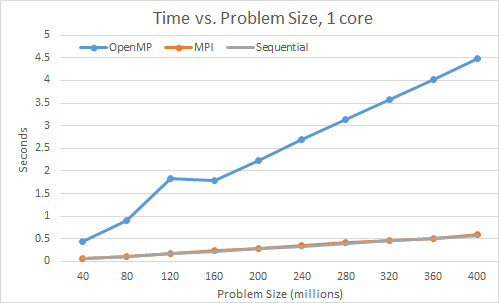
\includegraphics[width=1.0\textwidth]{figures/tvn_1.png}

	\caption{Time vs. $n$ on 1 core}
\end{figure}

The most noticeable feature of this data is the poor performance of the OpenMP algorithm.  Although it is expected that the parallel algorithms will perform worse than a sequential algorithm when only one core is utilized, the OpenMP algorithm shows a slowdown of at least 9 times, particularly with the largest problem size of 400 million.  After reviewing the code, however, it does not appear that there are glaring optimization issues.  This seems to suggest that the overhead of using OpenMP hurts it significantly with such a large problem size.

The MPI algorithm, on the other hand, works much better, and in fact its runtime closely resembles that of the sequential algorithm.

\begin{figure}[H]
	\centering

	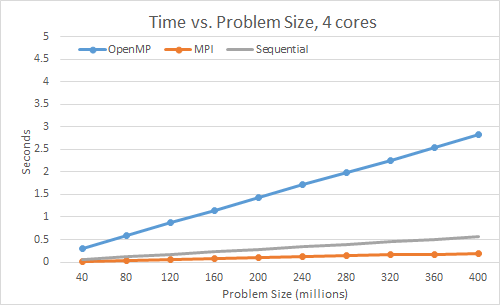
\includegraphics[width=1.0\textwidth]{figures/tvn_4.png}

	\caption{Time vs. $n$ on 4 cores}
\end{figure}

Perhaps more surpringly, even with 4 cores, the OpenMP algorithm cannot compete with the sequential algorithm.  Adding these extra cores do seem to help; the slowdown is closer to 6 times rather than 9.  However, it seems that the OpenMP algorithm shows such an intense slowdown with one core that adding more cores only helps the algorithm make up lost ground.

By contrast, the MPI algorithm behaves as expected, performing about 2-3 times faster than the sequential algorithm.

\begin{figure}[H]
	\centering

	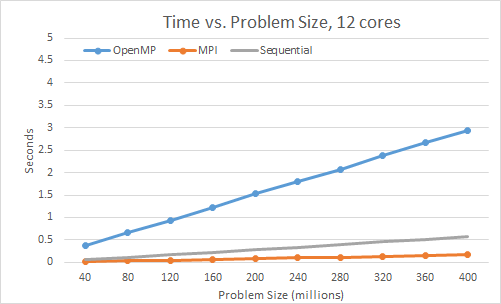
\includegraphics[width=1.0\textwidth]{figures/tvn_12.png}

	\caption{Time vs. $n$ on 12 cores}
\end{figure}

At this point, the OpenMP algorithm has completely stagnated.  Adding 8 more cores on top of the 4 cores from the previous figure does not make it run faster; in fact, it gets slightly \textit{worse}.  The MPI algorithm also stays around the same.  It can already be deduced from these graphs that neither algorithm experiences a near-ideal speedup, but this should be confirmed by the speedup chart. \\

The following figure combines the previous three figures for a side-by-side comparison:

\begin{figure}[H]
	\centering

	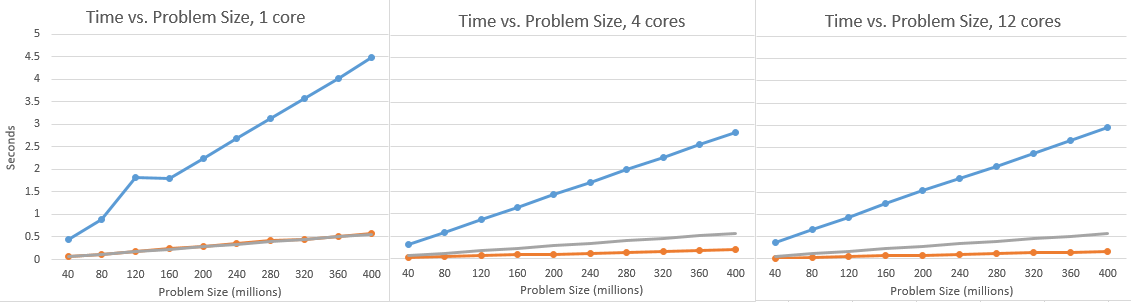
\includegraphics[width=1.0\textwidth]{figures/tvn_sidebyside.png}

	\caption{Side by side comparison of Time vs. $n$}
\end{figure}

\subsection*{Speedup}
\begin{figure}[H]
	\centering

	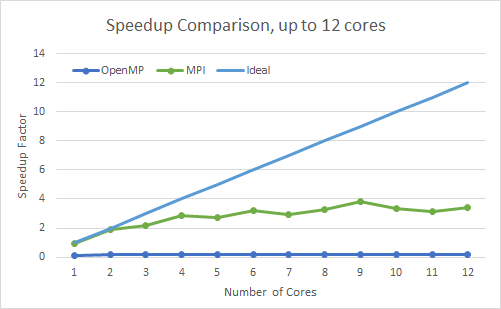
\includegraphics[width=1.0\textwidth]{figures/speedup.png}

	\caption{Speedup comparison between OpenMP and MPI}
\end{figure}

As expected, neither parallel algorithm experiences a particularly ideal speedup. The OpenMP algorithm in particular shows problematic performance.  Not only is it worse than the MPI algorithm, but its scaling factor is consistently less than 1, meaning it in fact is slower than the sequential algorithm no matter the number of cores.  The MPI algorithm fares much better, only dipping below 1 with one core.  As the number of cores approaches 12, the MPI algorithm settles on a speedup factor of roughly 2.5.


\subsection*{Scaling}

The following figure demonstrates the weak scaling factors of both the OpenMP and MPI algorithms when run on a single Westmere node.  The weak scaling factor compares the running time of a parallel algorithm on $n/p$ units per core versus the runtime of the sequential algorithm on $n/p$ units. The closer this scaling factor is to 1, the better.

\begin{figure}[H]
	\centering

	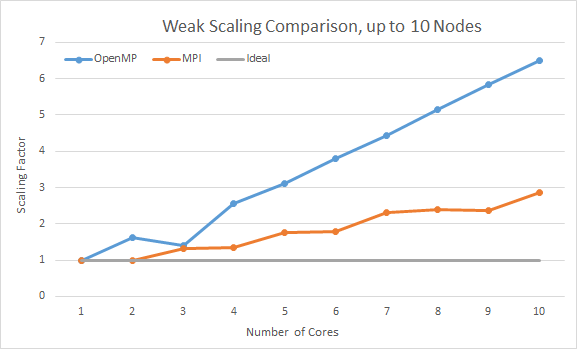
\includegraphics[width=1.0\textwidth]{figures/weakscaling.png}

	\caption{Weak Scaling comparison between OpenMP and MPI}
\end{figure}

For the OpenMP algorithm, not only does the scaling factor quickly diverge from 1 as the number of cores increases, but it increases at a constant rate, suggesting that the overhead required by OpenMP for adding cores is nonlinear.  The weak scaling factor of MPI also increases, but at a much lower rate (roughly one third that of OpenMP). \\

The next figure focuses on MPI exclusively, showing its strong scaling factor on a Nehalem node with much more than 10 cores.  Strong scaling is simply the ratio between the runtime of a parallel algorithm using $p$ cores vs. the runtime of the sequential algorithm on the same problem size.  If there are $p$ cores, the runtime would ideally be $1/p$ times the runtime of the sequential algorithm.  Thus, the ideal strong scaling line is $y=x$.

\begin{figure}[H]
	\centering

	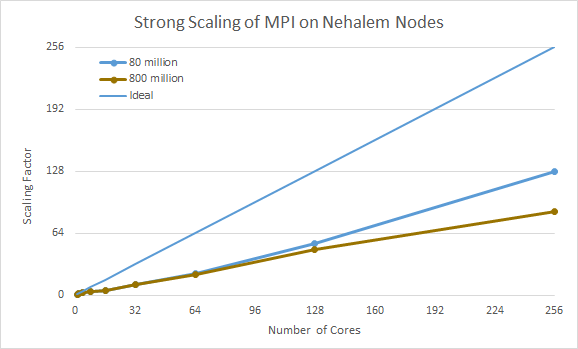
\includegraphics[width=1.0\textwidth]{figures/strongscaling.png}

	\caption{Strong Scaling analysis of MPI, on Nehalem nodes}
\end{figure}

For a problem size of 80 million, the strong scaling factor is roughly half of the ideal, which may still be considered a good scaling factor.  Also, the data suggests that as the problem size increases, there is a non-trivial effect that the resulting overhead of MPI has on the scaling factor.  However, for an order of magnitude jump in problem size, the above difference may also be considered reasonable.

\subsection*{Expected vs. Theoretical Performance}

Now, we shall determine whether the experimental results of all three algorithms match up with their corresponding theoretical complexities.  Recall the definition of big-O:

$$f(n) = O(g(n)) \implies 0 \leq f(n) \leq c \cdot g(n),\ \text{for all}\ n \geq n_0$$

For each of the three algorithms, we will find approximate values or bounds for $\mathbf{c}$ and $\mathbf{n_0}$.

\begin{figure}[H]
	\centering

	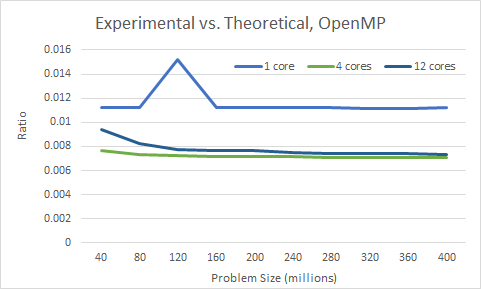
\includegraphics[width=1.0\textwidth]{figures/evt_omp.png}

	\caption{Expected vs. Theoretical ratio for OpenMP}
\end{figure}

The convergent nature of the above data supports the claim that the OpenMP algorithm runs in $O(n)$ time.  If the results did not fit the $O(n)$ model, we would observe a steady upward or downward change in the ratio as the problem size increased. \\

Our value of $\mathbf{c}$ can be found as the ratio value the graph converges to as the problem size increases.  For 1 core, we find that $c \approx 0.011$, but as the number of cores increases that value converges to $c \approx 0.0007$. \\

The value of $\mathbf{n_0}$ is the problem size at which the ratio begins to converge.  For OpenMP, there is some divergence up until 160 million, at which point the ratios all stay relatively stable.  Thus we will say that $n_0
\approx 160,000,000$.

\begin{figure}[H]
	\centering

	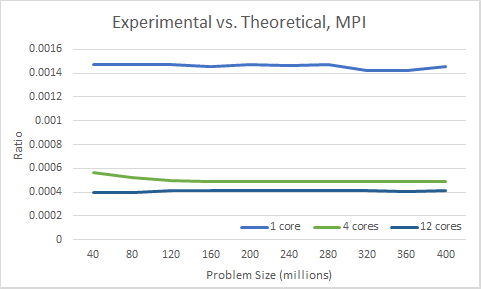
\includegraphics[width=1.0\textwidth]{figures/evt_mpi.png}

	\caption{Expected vs. Theoretical ratio for MPI}
\end{figure}

We will perform the same process on MPI.  For 1 core, $c = 0.0015$, but as the number of cores increases, we find that $c$ converges to roughly $0.0004$.  Our value of $n_0$ is more difficult to find, as it seems that the data is already rather convergent.  It is possible that $n_0$ is currently outside of our data range; therefore, we will simply establish a bound at $n_0 < 120,000,000$.

\begin{figure}[H]
	\centering

	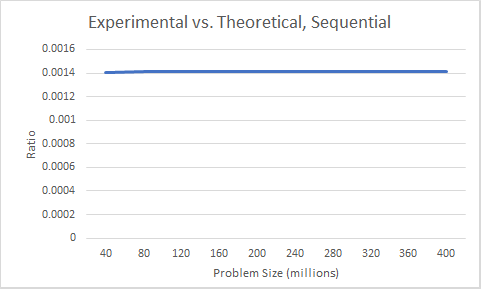
\includegraphics[width=1.0\textwidth]{figures/evt_seq.png}

	\caption{Expected vs. Theoretical ratio for sequential algorithm}
\end{figure}

The data for the sequential algorithm is practically constant, so we will say that $c \approx 0.0014$ and establish a bound for $n_0$ at $n_0 < 40,000,000$. \\

Overall, the charts for each of these algorithms support the claim that they run in $O(n)$ time.  Then, it would be meaningful to compare their values for $c$ ($n_0$ is slightly less important as it is much more hardware-dependent). Similar to the time vs. problem size chart, we see that the MPI and sequential algorithms share similar values for $c$; thus, we can say that their asymptotic rate of growth is similar.  OpenMP, on the other hand, has a value for $c$ that is more than ten times that of the MPI and sequential algorithms, supporting the claim that it simply grows faster, albeit with the same asymptotic complexity.

\section{Conclusion}
Ultimately, for large values of $n$, the MPI algorithm wins on all fronts.  Despite the need for inter-process communication, the algorithm presented has minimized the necessary overhead, and the benefits clearly show.  The OpenMP algorithm right now is rather lacking, and seems that it could use some optimization.  The expected vs. theoretical analysis of the OpenMP algorithm supports the claim that it is in fact running in $O(n \log n)$ time, and thus cannot win out against the $O(n)$ runtime of MPI or of the sequential algorithm.  Attempts at optimization were already made by modifying the OpenMP inner loop to use a bitwise operation instead of a power function.  This resulted in a marginal decrease in running time, but not by an order of magnitude. \\

Perhaps the OpenMP algorithm would be more useful at smaller problem sizes, where the speedup due to parallelization offsets the required overhead.  Unfortunately, given the current situation, it has not scaled well.  Another thing to take into consideration is that this algorithm is laid out by NVIDIA and is thus likely to be much more effective on a graphics card, with thousands of cores.  In that situation, perhaps the OpenMP algorithm would win out against an MPI implementation with the same number of cores.  That, however, cannot be confirmed without further experimentation.

So, the MPI algorithm is the ideal here in terms of performance with large problem sizes and a moderate number of cores.  On a system with only a few cores, or with smaller problem sizes, the sequential algorithm would likely be the better choice overall.  It has less overhead than both the OpenMP and MPI algorithms, not to mention its incredible simplicity.

\end{document}